
% Gender-inclusive: Relevant throughout the document but frequently occuring here:
% - [ ]  write gender-inclusive: do not use he or she but use they instead: "the participant was asking..., he liked ... → they liked (in singular)
% check for the following:
% - [ ]  Have you used “man” or “men” or words containing them to refer to people who may not be men?
% - [ ]  Have you used “he,” “him,” “his,” or “himself” to refer to people who may not be men?
% - [ ]  If you have mentioned someone’s sex or gender, was it necessary to do so?
% - [ ]  Do you use any occupational (or other) stereotypes?
% - [ ]  Do you provide the same kinds of information and descriptions when writing about people of different genders?

\section{User Study \& Methods}
We set out to answer three questions: First, can we tune haptic rendering to participants preferences using a reinforcement learning (RL) agent? Second, is it possible to rely on implicit labels obtained through a neural decoder? And third, what is the cost when relying on implicit instead of explicit labels?

To answer these questions, we designed a user study using a pick-and-place task in VR, where visual, auditory, and haptic sensations were differentially rendered during object pick-up. After obtaining labeled data and training a neural decoder, participants completed two blocks in which an RL agent tried to predict the haptic feedback participants seemed to find most realistic. In one block, the RL agent operated on participants' explicit ratings on a questionnaire, and in the other, it operated on the (implicit) output of the neural decoder.

% In a first study condition, participants were asked to rate the realism of the interaction. These explicit labels were used to train a decoder of interaction realism based on neural signals. In a second condition, participants again executed the pick-and-place task, this time without providing explicit labels about the interaction. In both conditions, an RL agent was employed to choose the preferred combination of sensory channels rendered for object pick-up, relying either on explicit (condition 1) or implicit labels (condition 2).
% To answer the last question, we defined the dependent variable cost as ...

\subsection{Participants} % TODO
17 participants (M = XX years, SD = YY) were recruited from our local institution and through the online participant pool of the institute. Participants were compensated with course credit or 12 Euro per hour of study participation. Before participating, they were informed of the nature of the experiment, recording, and anonymization procedures, and signed a consent form. The project was approved by the local ethics committee of the Department of Psychology and Ergonomics at the TU Berlin (Ethics protocol approval code: BPN\_GEH\_220421).

The first five participants only completed the \textit{training} part of the experiment, meaning they did not complete the two blocks with the RL agent. Hence, their data were used together with the remaining participants only for \todo{the analyses on X and Y}.

\subsection{Apparatus}
The experimental setup, depicted in Figure~\ref{fig:setup}, comprised: (1) a VR headset with a built-in eye tracker, (2) a haptic glove with an attached motion tracker, (3) a 64-channel EEG system and a VR capable computer. To assist readers in replicating our experiment, we provide the necessary technical details, the complete source code for the VR experiment, the collected data, and the analysis scripts~\footnote{\url{anonymized}}. % \todo{add link to github and data repository}.

\begin{figure}
    \centering
    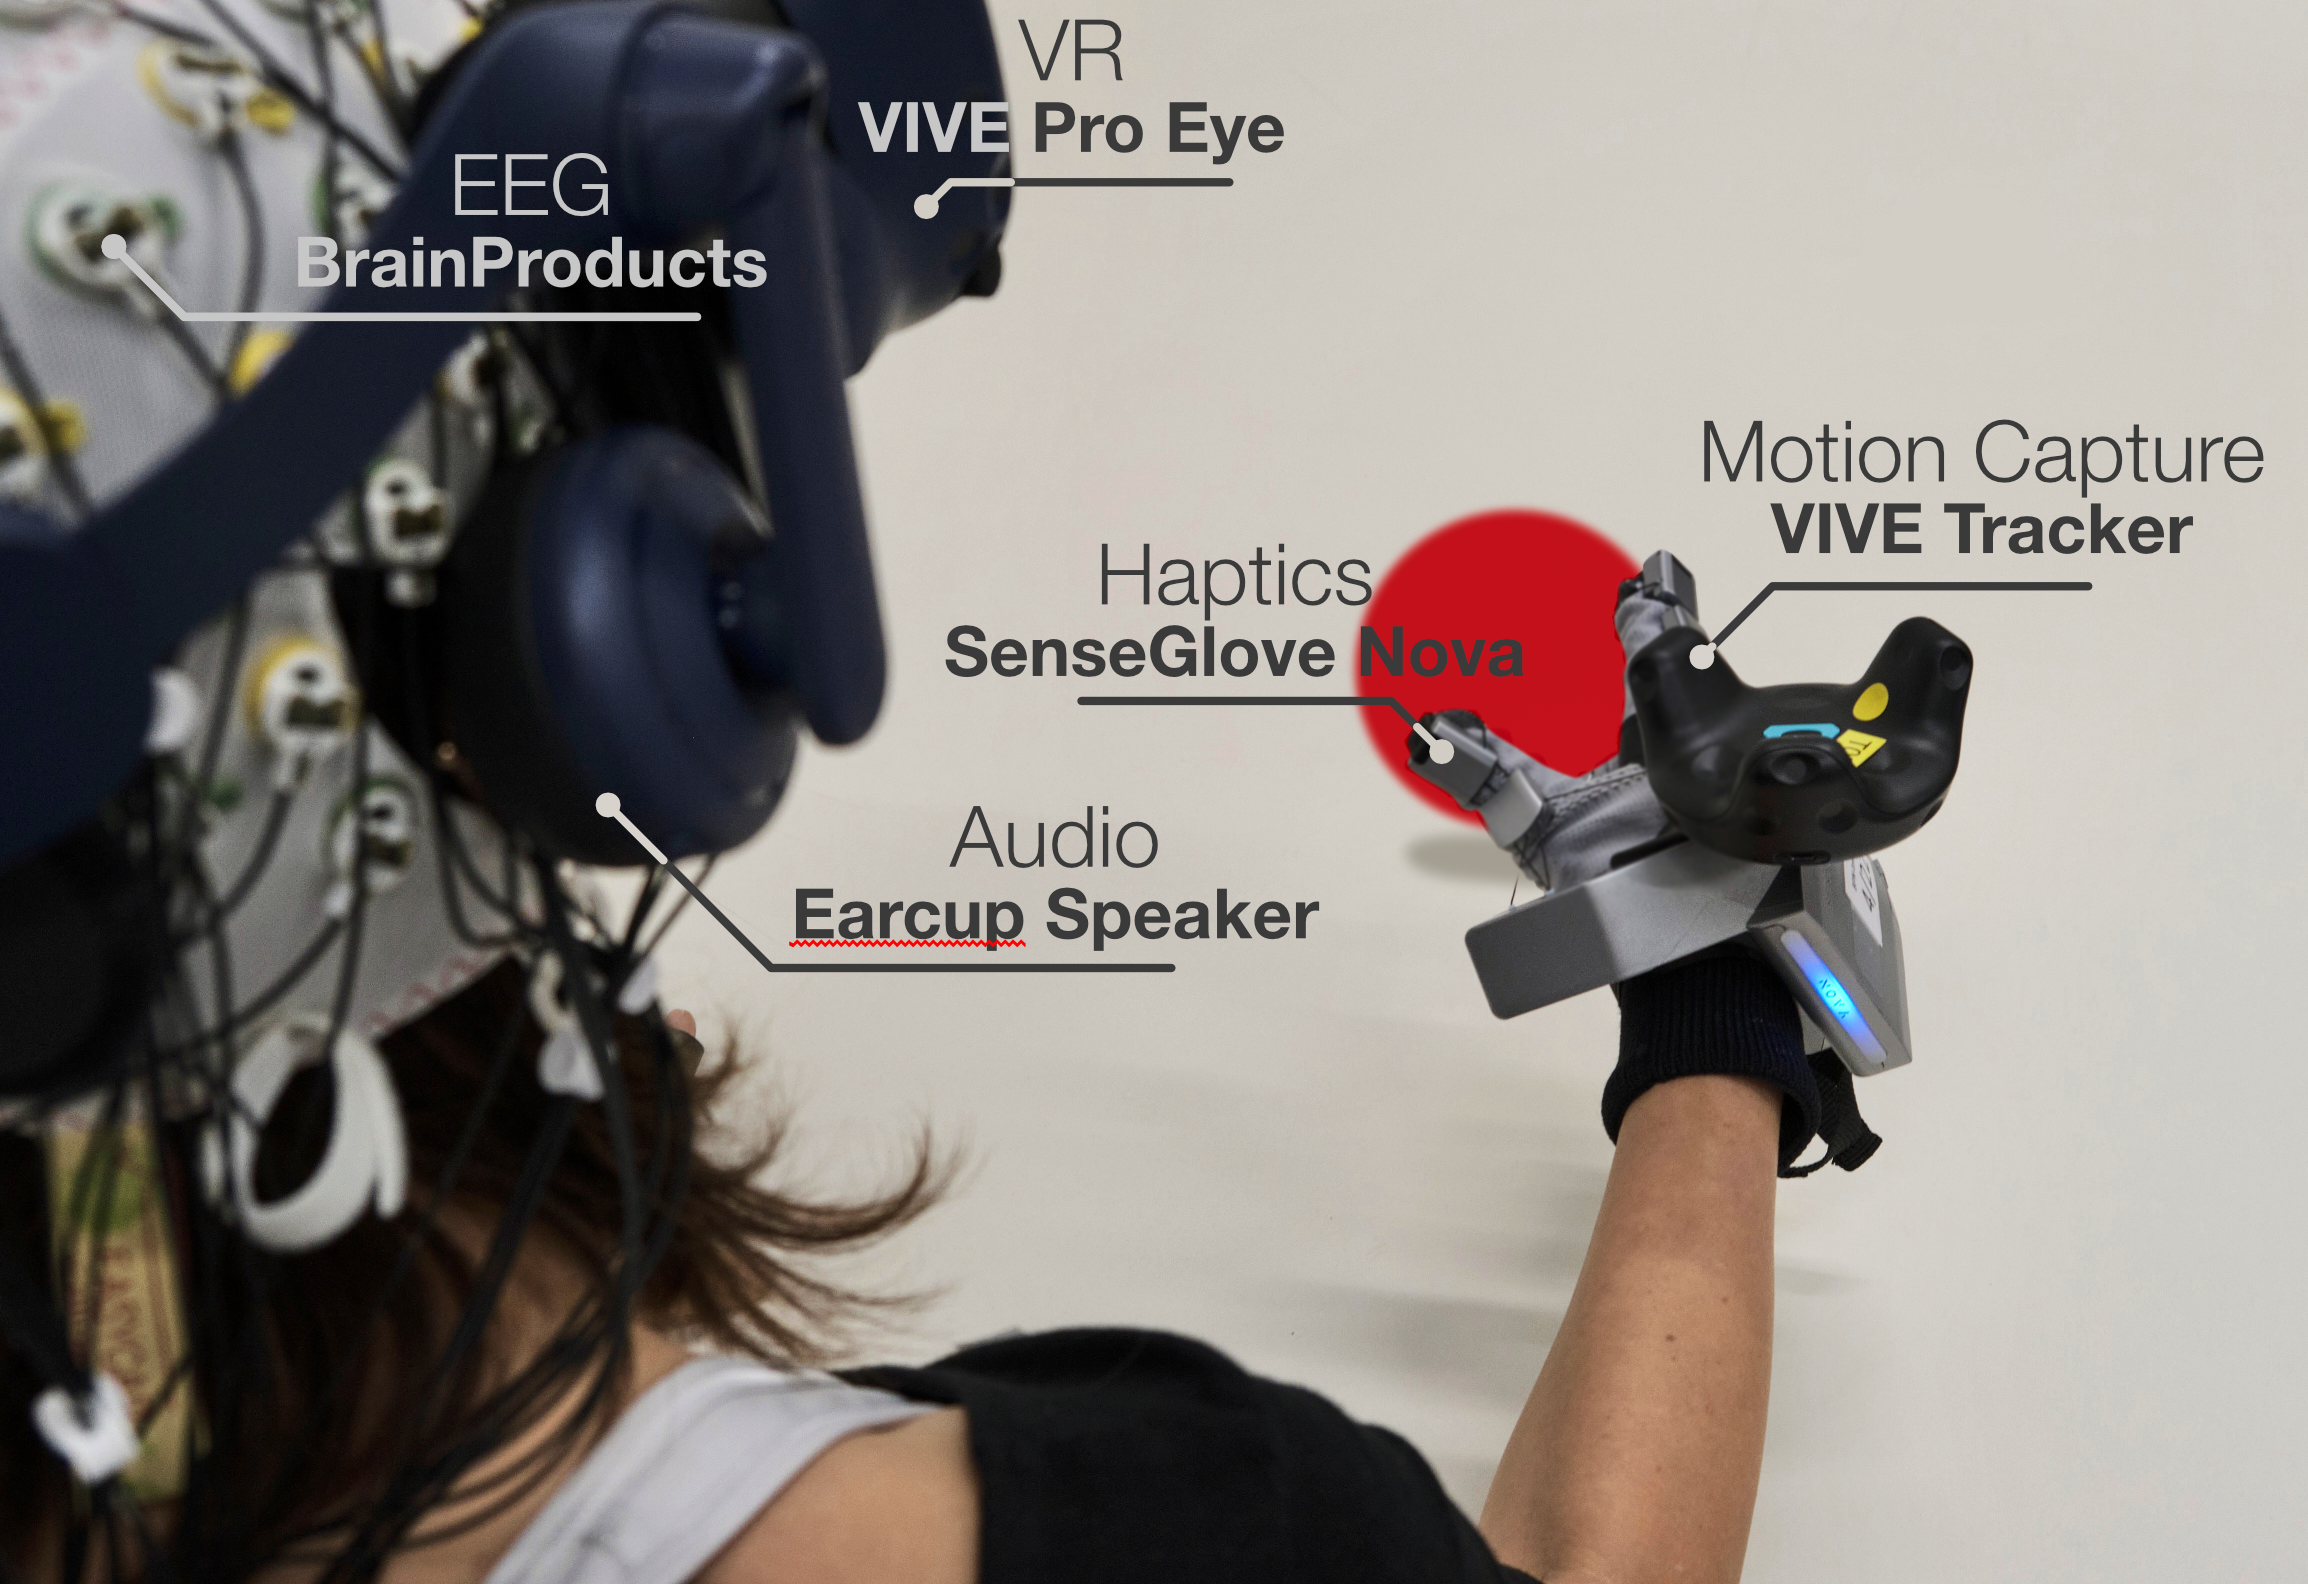
\includegraphics[width=\linewidth]{input/img/setup.png}
    \caption{Experimental setup featuring a participant equipped with EEG (BrainProducts), Head-mounted display (VIVE Pro Eye), haptic feedback (SenseGlove Nova), motion capture (VIVE Tracker), and audio output (earcup speaker).}
    \Description{Experimental setup integrating various technologies for virtual reality (VR), motion capture, haptics, audio feedback, and brain activity monitoring. The participant wears an EEG cap (BrainProducts) to record neural activity, a VIVE Pro Eye headset for immersive VR, and a SenseGlove Nova haptic glove with a VIVE Tracker for motion tracking. An earcup speaker provides audio feedback, enhancing the multisensory experience.}
    \label{fig:setup}
\end{figure}

\textbf{(1) VR.} We used an HTC Vive Pro Eye headset (HTC Corporation, Taiwan) to render the scene and sample eye-tracking using SRanipal (REF version?). We replaced the stock strap of the headset with the Vive Deluxe Audio Strap to ensure a good fit and reduce discomfort potentially caused by the EEG cap.

\textbf{(2) Haptic Glove.} The SenseGlove Nova V1.0 (SenseGlove, Netherlands) was used to sample finger movements and render vibro-tactile sensations. To track hand movements, an HTC Vive tracker was attached to the glove, as recommended by the manufacturer.

\textbf{(3) EEG Setup.} EEG data was recorded from 64 actively amplified electrodes using BrainAmp DC amplifiers (BrainProducts, Germany). Electrodes were placed according to the extended international 10–20 system~\cite{Jasper1983-uw}. One electrode was placed under the right eye to provide additional information about eye movements (vEOG). After fitting the cap, all electrodes were filled with conductive gel to ensure proper conductivity, and electrode impedance was brought below 10k$\Omega$ where possible. EEG data was recorded with a sampling rate of 250 Hz. 

We used `labstreaminglayer' (LSL)~\cite{Kothe2024-mx} to make data streams for the hand and eye motion, EEG data, and an experiment marker stream that marked sections of the study procedure available in the network. LSL's LabRecorder was used to collect data streams with timestamps.

\subsection{Task}
In the task, participants were instructed to pick up an object and then place it in a target location. They were instructed to be accurate while maintaining a steady pace. The object was placed on a table in front of them and for grabbing they used the grab functionality of the haptic glove. Successful grabbing required them to use all fingers, ensuring that both the thumb and at least one other finger securely held the object. After picking up the object, the participants moved it to the center of a sphere that visually indicated the location of the goal. Once the object was released, participants received feedback about their placement accuracy, displayed as a numerical value in centimeters on the table, indicating the distance between the object’s placement and the center of the goal sphere.

\todo{task procedure figure with screenshots, integrate with data flow diagram}
\begin{figure*}[!ht]
    \centering
    \includegraphics[width=\linewidth]{input/img/dataflow_experiment.pdf}
    \caption{Task and data flow in both, \textit{explicit} (top) and \textit{implicit} (bottom) experimental conditions.}
    \Description{Task and data flow in both, \textit{explicit} (top) and \textit{implicit} (bottom) experimental conditions.}
    \label{fig:dataflow}
\end{figure*}

Depending on the trial condition, see procedure below, participants were then asked to answer the question ``'' (translated) which was chosen from the \textit{Multimodal Presence Scale}~\cite{Makransky2017-hr}. The anchors of the question were ``'' and ``''. % todo add questionnaire anchor
To give their answer, participants could move a slider handle by grabbing it in the same way as they were grabbing the object in the task; see figure~\ref{fig:dataflow}.

\subsubsection{Interface Conditions}
The pick-and-place interaction was designed to simulate a multimodal interaction with visual, auditory, and haptic feedback. To this end, the following sensations were rendered:

\textbf{(1) Visual-only Baseline.} The object changed its color from white to red when it was grabbed.

\textbf{(2) Visual-only with Sound.} Together with the color change from white to red, a sound was played at 50\% volume through the Vive's earcup speakers. We used a simple `plop' like sound with a duration of 200 ms.

\textbf{(3) Visual-only with Vibrotactile.} With the color change, vibrotactile sensations were rendered at the tip of the thumb, index-- and middle finger, and the back of the hand. The vibrotactile profile was \todo{check unity again for the profile shape}

\textbf{(4) Visual-only with Sound and Vibrotactile.} Color change, sound, and vibrotactile feedback were rendered together.

\subsubsection{Procedure}
In total, participants completed three experimental blocks. In the first block, 140 trials had to be completed, with each interface condition being experienced 35 times. The order of the interface conditions was randomized. After every pick-and-place, the questionnaire was presented and participants had to give their rating of the preceding pick-and-place interaction. These labeled data were later used to train and assess the neural decoder.

After this first block, the features for the decoder were extracted from the EEG data, and the decoder was trained. This took about 5-10 minutes, during which participants could rest. Next, the two experimental conditions of interest were conducted. The order in which the conditions were tested was counterbalanced across participants. 

In the \textit{explicit} condition, participants rated every interaction using the slider. The slider values were extracted as 0--1 and fed forward to the RL agent, see \ref{RL} for technical details on the leveraged RL implementation. The agent then selected the interface condition of the next trial. In the \textit{implicit} condition, the question was omitted and instead the output from the decoder, after normalization to the 0--1 range, was fed to the agent. As in \textit{explicit}, the agent then selected the interface condition of the following trial. 

For both experimental conditions, we set the agent to stop after picking the same interface condition 5 times in a row, i.e. the \textit{convergence} criterion.

\subsection{Reinforcement Learning Agent}\label{RL}
%% ALEKS START %%


%% ALEKS END %%

% \subsubsection{Experimental Design \& Data Flow}

\subsection{Neural Signal Decoder}
For loading, synchronizing, and pre-processing the EEG data from the 140 trials of labeled training data, we utilized the EEGLAB~\cite{Delorme2004-sn} toolbox with wrapper functions from BeMoBIL-pipeline~\cite{Klug2022-lc} running in a MATLAB 2023b environment (The MathWorks Inc., USA).

Our goal was to design a general decoder of the expected haptic sensations in VR. Therefore, we presumed the most salient neural data to be present directly following the `haptic' event of picking up the object in our pick-and-place task. Hence, we extracted 1 s long data segments following this event and trained a binary model to score expected--unexpected sensations.

In the first step to prepare the data for classifier training, noisy trials were rejected. To this end, the EEGLAB function `autorej' was used on the EEG data, keeping the default parameters. Next, further trials were flagged and removed by detecting extreme outliers in participants behavior. We used Tukey's method~\cite{Tukey1949-sl} based on $1,5*IQR$ (Interquartile Range) to determine trials where participants behavior deviated significantly with respect to the placement accuracy of the target object. This resulted in the exclusion of a total XX (SD = YY) trials out of XX trials (X participants x Y conditions x Z trials).

Prior to feature extraction, the EEG data was band-pass filtered to retain frequencies from .1 to 15 Hz via Fast Fourier Transform (FFT).

\subsubsection{Features}
To obtain a robust classifier with many samples for training, we reduced the classification problem to a binary situation. Using a median split on the questionnaire ratings, we grouped all trials below the median into a \textit{mismatching expectation} class and all trials above into \textit{matching expectation}, resulting in a balanced dataset with two classes of equal size. 

The filtered data of all channels was then segmented into 12 epochs of interest of 50 ms size from 0--600 ms following the grab. The samples in each 50 ms segments were then aggregated using the mean, resulting in a matrix of 64 channels X 12 aggregated time windows. Next, baseline correction was performed by subtracting the first time, i.e. 0--50 ms after the grab. The first two time windows were discarded, resulting in a 64 X 10 matrix retained for each trial.

A paired t-test was performed for each feature (channel and time window) to identify the most discriminative features between the \textit{mismatching} and \textit{matching} conditions. The absolute value t-statistics were then sorted and stored. For each participant we performed a grid-search on the number of features to use for classification. To this end, the classifier accuracy was assessed at 10 to 100 features, increasing in steps of 5. The number of features resulting in a model with the highest accuracy was saved for real-time application. These models were always fit on 80\% of the data (80 -- 20 train-test split). To assess classifier performance, the following performance metrics were calculated: Accuracy, F1 score, and ROC.

We used a linear discriminant analysis (LDA) with shrinkage regularization (automatic shrinkage using the Ledoit-Wolf lemma~\cite{Ledoit2004-bi}) using the implementations from scikit-learn~\cite{Pedregosa2012-sj}. In order to normalize LDA scores during real-time application to the 0--1 range, we extracted the LDA scores of the 20\% test data held out during model fitting. Then, for min-max normalization, the 5th and 95th percentiles were taken from that distribution and stored for normalization of single trials during real-time application. This allowed us, to retrieve 0--1 values from single trials from the binary representation of matching vs. mismatching feedback expectations.

\subsubsection{Real-time Application}
During real-time application, the EEG data was buffered for one second following a grab. The data was band-pass filtered analogously to the training data from 0.1 to 15 Hz. Next, the features from the best performing model were extracted and, using that model, transformed to an LDA score. Using the min-max anchors, the score was normalized to the 0--1 range and sent to an LSL stream in order to be fetched by the RL agent.

\subsection{Hypotheses \& Statistical Testing}
To answer whether haptic rendering can be tuned using an RL agent, we checked whether the agent arrived at the \textit{true} label. The true label was operationalized by selecting the interface condition with the highest mean rating in block 1, the training data. An exact McNemar's test~\cite{McNEMAR1947-bp} was conducted on the contingency table on matching both explicit and implicit convergence to the true label, see figure~\ref{res:cm_table}. We hypothesized that both explicit and implicit feedback result in the same performance and hence that the test shows no effect.

Next, we hypothesized that, irrespective of feedback origin, the RL agent requiring the same number of steps until convergence. As a reminder, the agent finished picking when it chose the same label 5 times in a row. A paired \textit{ttest} was conducted comparing the number of steps until convergence with implicit vs. explicit feedback.
% NOTE: is it necessary to mention that it stopped picking after 100 trials? See if this ever happens in the final data